\documentclass{beamer}
\usepackage{hyperref}
\usepackage[T1]{fontenc}
\usepackage{PekingU}
\hypersetup{colorlinks=true,urlcolor=cyan,linkcolor=peaking}

% other packages
\usepackage{latexsym,amsmath,xcolor,multicol,booktabs,calligra}
\usepackage{graphicx,pstricks,listings,stackengine}

\author{Gabriel Wu (@lucifer1004)}
\title{When Taichi meets Julia}
\subtitle{A short introduction to Taichi.jl}
\date{\today}

% defs
\def\cmd#1{\texttt{\color{red}\footnotesize $\backslash$#1}}
\def\env#1{\texttt{\color{blue}\footnotesize #1}}
\definecolor{deepblue}{rgb}{0,0,0.5}
\definecolor{deepred}{rgb}{0.6,0,0}
\definecolor{deepgreen}{rgb}{0,0.5,0}
\definecolor{halfgray}{gray}{0.55}

\lstset{
    basicstyle=\ttfamily\small,
    keywordstyle=\bfseries\color{deepblue},
    emphstyle=\ttfamily\color{deepred},    % Custom highlighting style
    stringstyle=\color{deepgreen},
    numbers=left,
    numberstyle=\small\color{halfgray},
    rulesepcolor=\color{red!20!green!20!blue!20},
    frame=shadowbox,
}


\begin{document}
\begin{frame}
    \titlepage
    \begin{figure}[htpb]
        \begin{center}
            
\includegraphics[width=0.5\linewidth]{pic/taichi.png}
            
\includegraphics[width=0.2\linewidth]{pic/julia.png}
        \end{center}
    \end{figure}
\end{frame}

\begin{frame}
    \tableofcontents[sectionstyle=show,subsectionstyle=show/shaded/hide,subsubsectionstyle=show/shaded/hide]
\end{frame}

\section{Why Taichi.jl?}
\begin{frame}{Why Taichi.jl?}
    \begin{columns}
        \column{0.4\textwidth}
        \centering
        \begin{itemize}
            \item I love Julia...
            \item I love Taichi...
            \item Why not both?
        \end{itemize}
        \column{0.6\textwidth}
        \centering
        \begin{figure}[htpb]
            \begin{center}
                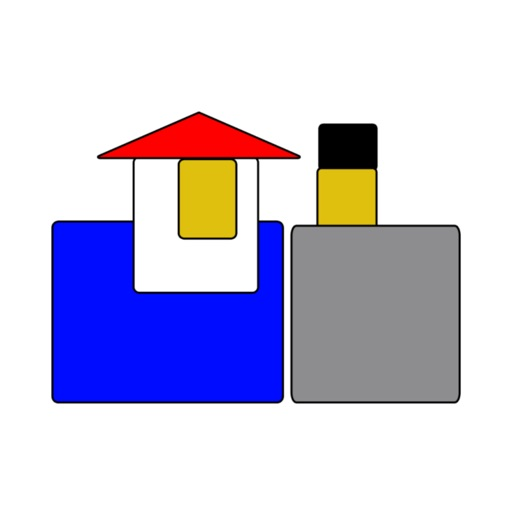
\includegraphics[width=\linewidth]{pic/wantboth.jpg}
            \end{center}
        \end{figure}
    \end{columns}
\end{frame}

\section{How I made Taichi.jl}
\begin{frame}[allowframebreaks]{First attempt}
    Using \texttt{PythonCall.jl}, most methods of \texttt{Taichi} can be directly called:
    \begin{figure}[htpb]
        \begin{center}
            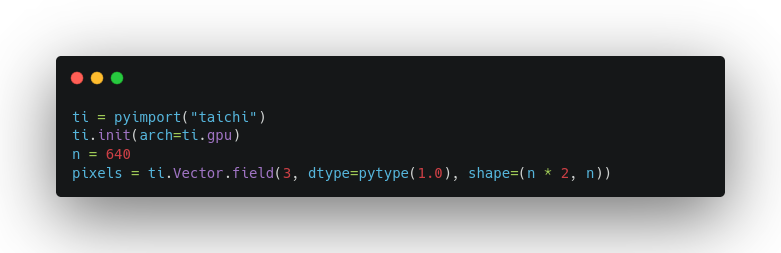
\includegraphics[width=\linewidth]{pic/code_01.png}
        \end{center}
    \end{figure}

    \framebreak
    However, the following would fail:
    \begin{figure}[htpb]
        \begin{center}
            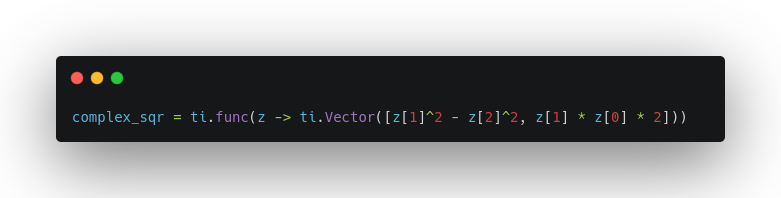
\includegraphics[width=\linewidth]{pic/code_02.png}
        \end{center}
    \end{figure}
    Because when \texttt{PythonCall.jl} passes a Julia function to Python, it is more like a pointer and Python will not know much about inside the function. But \texttt{Taichi} needs even the source code of the function to generate and transform the AST.
\end{frame}

\begin{frame}{Second attempt}
    We could write the function in Python, and the following worked!
    \begin{figure}[htpb]
        \begin{center}
            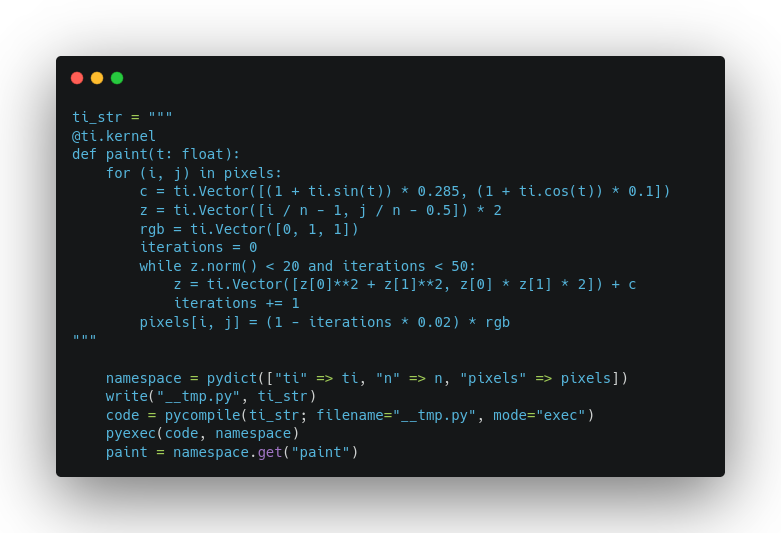
\includegraphics[width=.8\linewidth]{pic/code_03.png}
        \end{center}
    \end{figure}
\end{frame}

\begin{frame}[allowframebreaks]{Third attempt}
    Not elegant, though. Can't we just write the function in Julia?

    Here is another Julia package by me, \href{https://github.com/lucifer1004/Jl2Py.jl}{\texttt{Jl2Py.jl}}:

    \begin{figure}[htpb]
        \begin{center}
            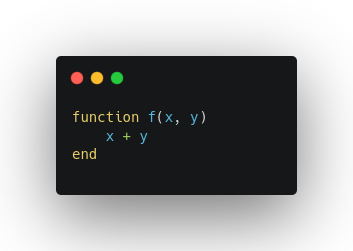
\includegraphics[width=.45\linewidth]{pic/code_04.png}
            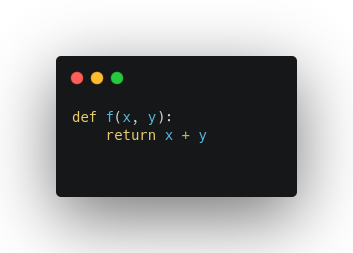
\includegraphics[width=.45\linewidth]{pic/code_05.png}
        \end{center}
    \end{figure}

    \framebreak

    Success!
    \begin{figure}[htpb]
        \begin{center}
            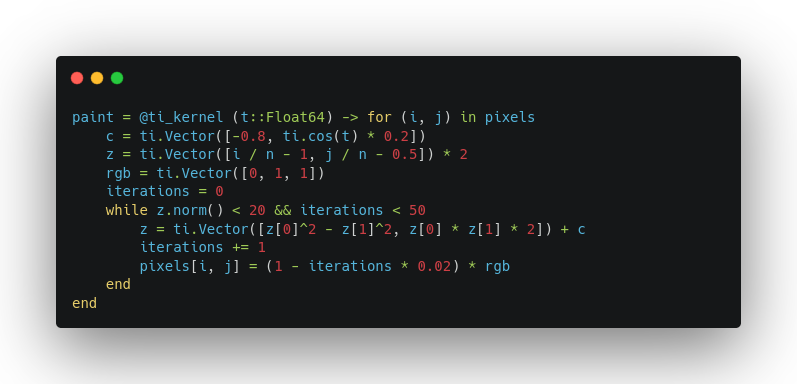
\includegraphics[width=.8\linewidth]{pic/code_06.png}
        \end{center}
    \end{figure}

    \framebreak
    And I have published it as a Julia package: \href{https://github.com/lucifer1004/Taichi.jl}{Taichi.jl}

    \begin{figure}[htpb]
        \begin{center}
            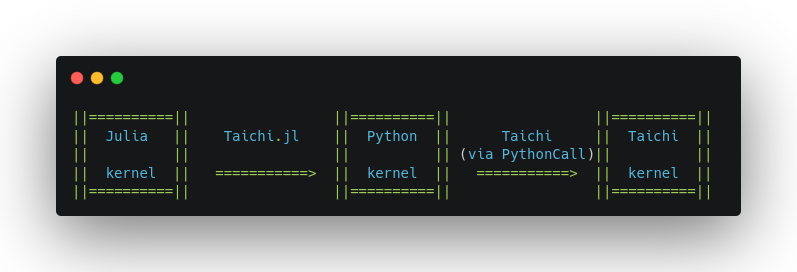
\includegraphics[width=.8\linewidth]{pic/code_07.png}
        \end{center}
    \end{figure}
\end{frame}

\section{Example usage of Taichi.jl}
\begin{frame}{Julia Set}
    \begin{figure}[htpb]
        \begin{center}
            
\includegraphics[width=.8\linewidth]{pic/juliaset.png}
        \end{center}
    \end{figure}
\end{frame}

\begin{frame}{Game of Life}
    \begin{figure}[htpb]
        \begin{center}
            
\includegraphics[width=.6\linewidth]{pic/gameoflife.png}
        \end{center}
    \end{figure}
\end{frame}

\begin{frame}{uFDTD}
    This example lies in \href{https://github.com/lucifer1004/uFDTD-Taichi}{lucifer1004/uFDTD-Taichi}

    \begin{figure}[htpb]
        \begin{center}
            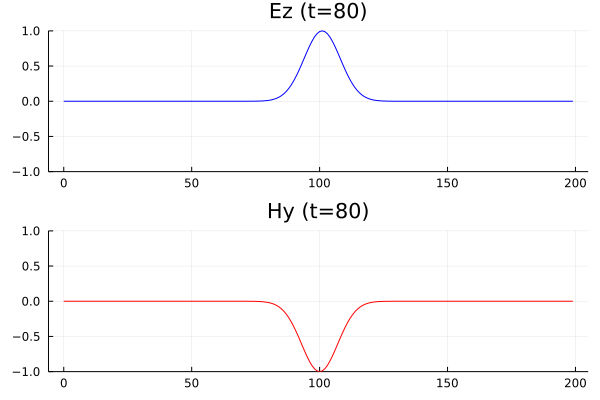
\includegraphics[width=.8\linewidth]{pic/1d_tfsf.png}
        \end{center}
    \end{figure}
\end{frame}

\section{The Future}
\begin{frame}{The Future}
    \begin{itemize}
        \item Bypass Python:

              Transpile directly from Julia AST to Taichi AST
        \item Memory share:

              Share device memory between Julia and Taichi
    \end{itemize}
\end{frame}

\begin{frame}
    \begin{center}
        {\Huge\calligra Thanks!}
    \end{center}
\end{frame}

\end{document}
